% DinoVision paper-section freeze candidate, 2026-08-02 America/Los_Angeles.

\subsection{Application-scale train-to-deploy case study: DinoVision}
\label{sec:dinovision}

We evaluate \system{} beyond isolated operators with DinoVision, an Android XR
application that reconstructs passthrough imagery from intermediate
DINOv3~\cite{simeoni2025dinov3} features
(Figure~\ref{fig:dinovision-quest3s}). The application center-crops and resizes
an RGB frame to $224\times224$, executes the first three layers of a frozen
DINOv3 ViT-S/16 encoder, rearranges its
$14\times14\times384$ patch features, and decodes them to RGB. On device, the
encoder and decoder form one batch-one inference graph, and two asynchronous
eye sessions share Blade's Vulkan context and queue with OpenXR rendering.

This case study exercises patch projection, learned prefix tokens, axial RoPE,
multi-head attention, LayerNorm, GELU MLPs, LayerScale, residual connections,
convolution, group normalization, SiLU, upsampling, autodiff, Adam, parameter
serialization, Android cross-compilation, and compute/graphics co-tenancy. It
is evidence about stack breadth and deployment closure, not a matched PyTorch
comparison or a capture-to-photon measurement.

\begin{figure}[t]
  \centering
  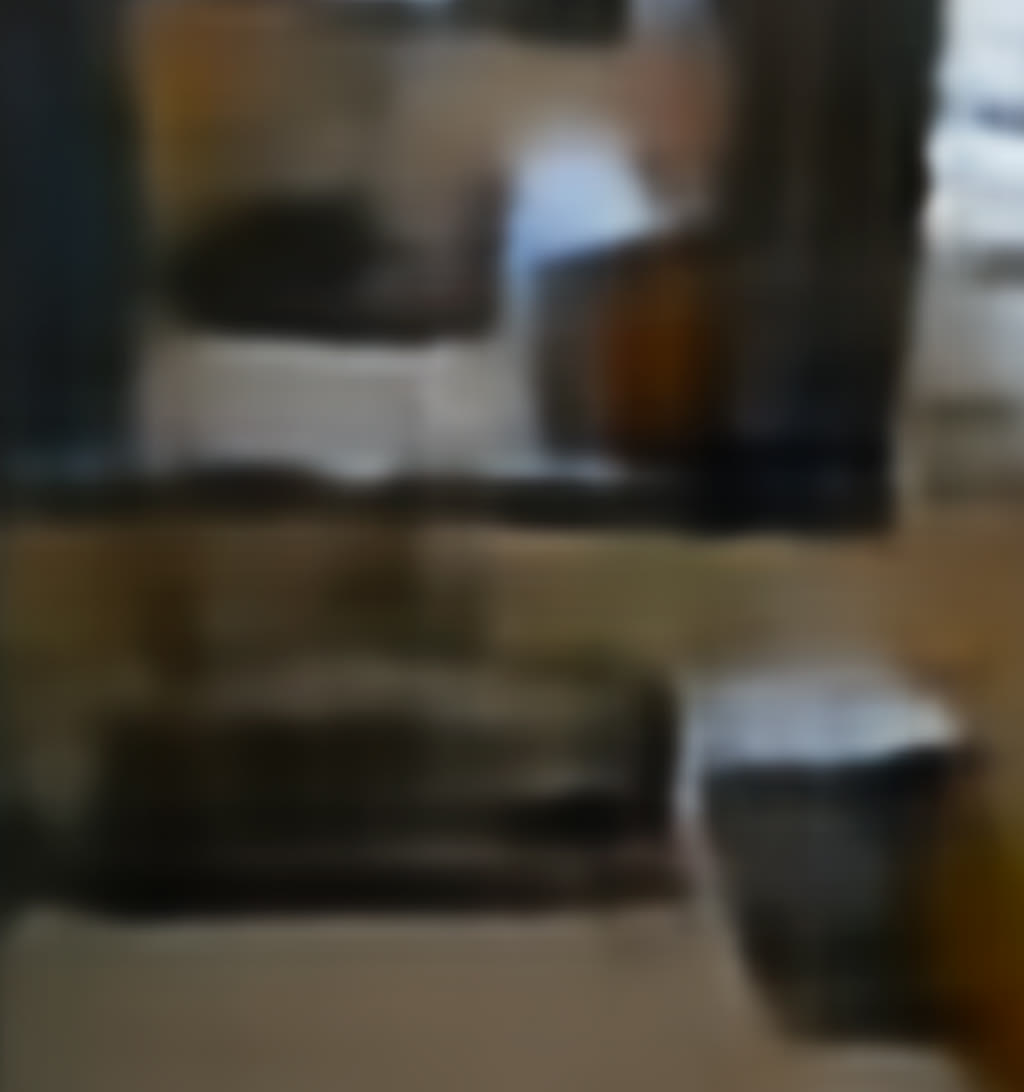
\includegraphics[width=0.82\columnwidth]{figures/dinovision-quest3s.jpg}
  \caption{Quest 3S casting capture of DinoVision's live RGB reconstruction.
  This qualitative image documents physical deployment; the correctness and
  timing claims use the protocols described below.}
  \label{fig:dinovision-quest3s}
\end{figure}

\paragraph{Host training and held-out evaluation.}
The frozen encoder caches features on an NVIDIA host, after which \system{}
trains a 2,012,547-parameter decoder-only batch graph. Deployment uses the same
decoder construction and learned parameters in a joined batch-one graph. The
paths therefore share graph operators, compiler, memory planner, and runtime,
but are not literally the same complete graph.

We preserve Imagenette's upstream split. Three independently initialized
runs each use a class-balanced 2,500-image training subset, 12,000 batch-eight
Adam updates, and all 3,925 validation images. Seed zero was selected for
deployment before validation; seed one later scored highest. Across seeds,
global validation PSNR is $21.86\pm0.11$ dB, median-image PSNR is
$22.45\pm0.12$ dB, median RGB SSIM is $0.6405\pm0.0076$, and median MAE is
$0.04672\pm0.00070$ (mean $\pm$ sample standard deviation). The public
artifact retains every per-image record; host wall time is excluded because
the interactive machine experienced recorded suspension gaps.

\paragraph{Independent correctness gate.}
The independent gate proved necessary: an initial LayerScale layout mismatch
updated only the first token even though the output images remained plausible.
We rejected all affected weights and measurements, corrected the layout,
added exact attention and LayerScale CPU tests, and retrained all replicates.

An independent Torch/Transformers reference and \system{} consume the same
normalized f32 tensor and checkpoint. Predeclared thresholds are relative
$L_2\leq0.01$, CLS cosine $>0.999$, and every patch-token cosine $>0.999$.
Table~\ref{tab:dinovision-correctness} shows that the deployed and full-depth
controls pass.

\begin{table}[t]
  \centering
  \footnotesize
  \setlength{\tabcolsep}{4pt}
  \caption{\system{} encoder agreement with the independent reference.}
  \label{tab:dinovision-correctness}
  \begin{tabular}{rccc}
    \toprule
    Encoder depth & Relative $L_2$ & CLS cosine & Worst patch cosine \\
    \midrule
     1 & 0.000781 & 1.000000 & 0.999989 \\
     3 & 0.001403 & 1.000000 & 0.999995 \\
    12 & 0.002253 & 0.999998 & 0.999995 \\
    \bottomrule
  \end{tabular}
\end{table}

\paragraph{Physical Android correctness.}
Before timing, the host and Quest execute one public fixed RGB frame with
identical encoder and preselected decoder weights. Preprocessed patches are
bit-exact. Encoder output has relative $L_2=0.001059$, cosine $0.999999441$,
and minimum token cosine $0.999973147$; spatial decoder input has relative
$L_2=0.001063$ and cosine $0.999999438$; reconstruction has relative
$L_2=0.000457$ and cosine $0.999999938$.

\paragraph{Submission chunking under graphics co-tenancy.}
A native benchmark first measures the joined 2.359-GMAC graph in isolation.
Each chunk cell retains 20 synchronized samples after five warmups in three
fresh processes. We then run a live-worn stereo OpenXR sweep for 90 seconds
per cell at inference interval zero. Both sweeps use the predeclared order
$4,16,1,12,2,8$ to expose time drift. Table~\ref{tab:dinovision-chunks}
reports application render submissions, not compositor/display rate; worker
latency is not capture-to-photon latency. After discarding two initial
five-second windows, every cell retains 16 windows. All state snapshots report
an awake, worn headset and thermal status zero; peak reported GPU temperature
is $63.9\,^{\circ}$C.

\begin{table*}[t]
  \centering
  \caption{Isolated submission cost and live Blade/OpenXR co-tenancy on Quest
  3S. Brackets are interquartile ranges; overhead is relative to one chunk.}
  \label{tab:dinovision-chunks}
  \begin{tabular}{rrrrr}
    \toprule
    Chunks & Isolated ms [IQR] & Overhead & Render submit Hz &
    Lower-eye Hz / worker ms [IQR] \\
    \midrule
     1 & 96.78 [96.02, 97.41] & baseline & 10.83 & 5.99 / 149.51 [148.37, 150.99] \\
     2 & 100.79 [99.78, 101.46] & +4.1\% & 12.87 & 6.51 / 119.25 [118.73, 119.84] \\
     4 & 105.76 [104.75, 107.49] & +9.3\% & 12.07 & 6.06 / 129.69 [128.11, 142.42] \\
     8 & 108.25 [107.33, 109.99] & +11.9\% & 12.70 & 6.37 / 128.94 [127.26, 130.13] \\
    12 & 112.91 [112.06, 114.43] & +16.7\% & 12.61 & 6.33 / 131.57 [126.65, 134.12] \\
    16 & 114.68 [113.67, 115.48] & +18.5\% & 11.87 & 5.94 / 143.37 [140.24, 145.27] \\
    \bottomrule
  \end{tabular}
\end{table*}

Chunking incurs monotonic isolated cost, reaching 18.5\% at 16 chunks. Under
live co-tenancy, two chunks instead improve render submissions by 18.8\% and
the lower-eye update rate by 8.7\%, while reducing median worker latency by
20.2\% relative to one chunk. Larger counts regress non-monotonically, so the
result establishes chunking as a measurable, caller-selected scheduling
control rather than a universal two-chunk optimum. The current runtime
partitions ordered compiler barrier groups evenly by count; it does not
estimate their duration or observe renderer latency.

The experiment does not measure on-device training, PyTorch-on-Android
speedup, quantitative headset-camera quality, or capture-to-photon latency.
The current path includes CPU camera conversion and patchification, explicit
GPU transfers, output readback, temporal smoothing, and renderer upload.
Full weights, raw samples, manifests, environment records, and validation
scripts are available at
\url{https://huggingface.co/mad-bot/dinovision}; source is available at
\url{https://github.com/kvark/dinovision}. The artifact also provides the
full-resolution casting captures and a 39-second live video.
